%!TEX root = index.tex
\chapter{Desenvolvimento da biblioteca} % (fold)
\label{cha:desenvolvimento_da_biblioteca}

\section{Recursos acadêmicos} % (fold)
\label{sec:recursos_acad_micos}

A principal contribuição da Escola Politécnica para o projeto veio das disciplinas de programação para automação (PMR2300 -- Computação para Automação e PMR2440 -- Programação para Automação) e de banco de dados (PMR2490 -- Sistemas de Informação). Além disso, a disciplina optativa PMR2728 -- Teoria de Probabilidades em Inteligência Artificial e Robótica abordou a temática do aprendizado de máquina e dos sistemas de recomendação.

Além das disciplinas do curso de Engenharia Mecatrônica, diversos recursos extra-curriculares foram de fundamental importância para o sucesso deste trabalho. Foram aplicados aprendizados práticos de quatro cursos da plataforma online Coursera (\url{https://www.coursera.org/}), sejam relacionados a teoria dos sistemas de recomendação, sejam relacionados a configuração de servidores na Amazon Web Services.

O curso ``Redes: Amigos, Dinheiro e Bytes'' (Networks: Friends, Money, and Bytes -- \url{https://www.coursera.org/course/friendsmoneybytes}), teve papel importante na introdução a temas ligados à rede mundial de computadores. Mais especificadamente, a aula 4 aborda, de maneira simples mas repleta de exemplos, a temática de sugestão de itens através da pergunta ``Como o Netflix recomenda filmes?''. Essa aula ajudou-nos a compreender a teoria por trás do algoritmo de recomendação do Netflix detalhado na Referência \citeonline{lops2011content-chap5}.


Outro curso que influenciou diretamente o nosso Trabalho de Conclusão de Curso foi ``Computação para Análise de Dados'' (Computing for Data Analysis -- \url{https://www.coursera.org/course/compdata}). As quatro semanas de aula ensinaram a leitura de dados formatados em R, o tratamento de dados, o uso de modelos estatísticos, como por exemplo métodos de regressão linear e polinomial, a aplicação de cálculos vetorizados e a construção de gráficos e tabelas. 

Aliado a essas aulas, aprendemos também o paradigma funcional, amplamente utilizado em R, durante as sete semanas de ``Princípios de Programação Funcional em Scala'' (Functional Programming Principles in Scala -- \url{https://www.coursera.org/course/progfun}). Todo o pacote foi construído em torno desse padrão de programação, visto que usuários de bibliotecas desejam utilizar métodos e funções genéricas para construção de resultados específicos.

Por fim, o curso de doze semanas de duração ``Engenharia de Startup'' (Startup Engineering -- \url{https://www.coursera.org/course/startup}) nos ensinou a trabalhar com diversas ferramentas de software necessárias para a realização dos testes de desempenho dos algoritmos. Utilizamos máquinas virtuais, linha de comando Unix, versionamento de código em \texttt{git} e editores de texto sem interface gráfica (tais como vi e Emacs). Além disso, o \textit{setup} de máquinas virtuais na Amazon Web Services também era abordada no curso, facilitando a configuração do ambiente de testes e a automatização desse processo. 

\section{Ferramentas utilizadas} % (fold)
\label{sec:ferramentas_utilizadas}

A programação da biblioteca computacional se deu por meio do ambiente de desenvolvimento integrado RStudio versão 0.98.953 (\url{http://www.rstudio.com/}). Esse IDE inclui console, editor de texto e corretor de sintaxe que suporta a execução de código direta, bem como ferramentas para traçar gráficos, histórico de comandos, depuração de erros e gerenciamento de espaço de trabalho. Além disso, o RStudio está disponível via licença de código aberto AGPLv3 (Affero General Public License version 3) para os principais sistemas operacionais (Windows, Mac e Linux).

\section{Métodos computacionais} % (fold)
\label{sec:m_todos_computacionais}



\subsection{Estrutura da biblioteca} % (fold)
\label{sub:estrutura_da_biblioteca}

A biblioteca está estruturada em quatro seções principais: \texttt{db}, onde está o banco de dados MovieLens 100k, \texttt{methods}, onde estão os algoritmos de recomendação, \texttt{results}, onde estão os métodos de avaliação de qualidade e \texttt{setup}, onde estão codificadas funções diversas, tais como leitura de banco de dados e cálculo de medidas de distância.

\begin{lstlisting}[caption=Estrutura da biblioteca]
recsys/
|-- db
|   `-- ml-100k
|       |-- u.data
|       |-- u.item
|       |-- u.user
|       |-- ...
|-- methods
|   |-- common
|   |   `-- up_ui_w.R
|   |-- fw.R
|   |-- ui.R
|   `-- up.R
|-- results
|   |-- benchmark.R
|   |-- performance.R
|   `-- run_tests.R
`-- setup
    |-- functions.R
    `-- setup.R
\end{lstlisting}

As principais funções da biblioteca estão descritas na documentação do Apêndice \ref{cha:documenta_o_da_biblioteca}, e o código pode ser obtido através do endereço \url{https://github.com/aviggiano/tcc/tree/master/recsys}.

% subsection estrutura_da_biblioteca (end)

\subsection{Algoritmo baseado na ponderação de atributos (FW)} % (fold)
\label{sub:algoritmo_baseado_na_pondera_o_de_atributos_fw_}

O algoritmo de ponderação de atributos possui cinco etapas: 

\subsubsection{Determinação de $e_{ij}$} % (fold)
\label{ssub:determina_o_de_e__ij_}

Em forma matricial, a Equação \ref{eq:determinacao-eij} pode ser descrita da forma \ref{eq:eij_matricial}.

\begin{equation}
\label{eq:eij_matricial}
\mathbf{E} = \mathrm{b}_M\left(\mathbf{R}^T\right) \mathrm{b}_M\big(\mathbf{R}\big)
\end{equation}

Em R, isso se traduz por uma simples instrução:

\begin{lstlisting}[caption=Determinação de $e_{ij}$]
e = b(t(r),M) %*% b(r,M)
\end{lstlisting}


\subsubsection{Determinação de $d_{ij}^f$} % (fold)
\label{ssub:determina_o_de_d__ij_f_}

Para o cálculo genérico de FW, a medida de distância padrão utilizada é a distância $L_1$ entre as duas \textit{features} (Equação \ref{eq:dijf2}, Código \ref{lst:dijf2}). Para o cálculo específico do banco de dados 100k-IMDB, as medidas de distância (Equação \ref{eq:dijf_especifico}, Código \ref{lst:dijf_especifico}) são determinadas segundo a Tabela TODO. 

\begin{equation}
\label{eq:dijf2}
d_{ij}^f = \left|a_{if} - a_{jf}\right|
\end{equation}

\begin{lstlisting}[caption=Determinação de $d_{ij}^f$ genérico,label=lst:dijf2]
d[i,j,] = abs(a[i,]-a[j,])
\end{lstlisting}

\begin{equation}
\label{eq:dijf_especifico}
\begin{split}
d_{ij}^f &= \left|a_{if} - a_{jf}\right|,~f \in \left\{1,21,23,24,25\right\} \\
d_{ij}^f &= J(a_{if},a_{jf}),~f = 2, \cdots, 20
\end{split}
\end{equation}


\begin{lstlisting}[caption=Determinação de $d_{ij}^f$ específico,label=lst:dijf_especifico]
d[i,j,1] = abs(a[i,21]-a[j,21])  
d[i,j,2] = abs(a[i,22]-a[j,22])  
d[i,j,3] = abs(a[i,23]-a[j,23])  
d[i,j,4] = abs(a[i,24]-a[j,24])  
d[i,j,5] = abs(a[i,25]-a[j,25])  
d[i,j,6] = abs(a[i,1]-a[j,1])    
d[i,j,7] = 1-jaccard(a[i,2:20],a[j,2:20])
\end{lstlisting}

\subsubsection{Determinação de $w_f$} % (fold)
\label{ssub:determina_o_de_w_f_}

O vetor $\mathbf{w}$ é obtido através da regressão linear de Equação \ref{eq:determinacao-wf}. Na linguagem R, basta aplicar o método \texttt{lm}, conforme  o Código \ref{lst:wf}.


\begin{lstlisting}[caption=Determinação de $w_f$,label=lst:wf]
# linear fit e ~ w0 + w (1-d)
D = 1-d
lm.W = lm(e ~ D, x=FALSE, y=FALSE, model=FALSE, qr=FALSE)
W = as.vector(lm.W$coefficients)
\end{lstlisting}

\subsubsection{Determinação de  $s_{ij}$} % (fold)
\label{ssub:determina_o_de_s__ij_}

Para o cálculo da matriz de similaridade, escolhemos os pesos $w_f>0$ e aplicamos a Equação \ref{eq:sij}, para todo $f>0$.

\begin{lstlisting}[caption=Determinação de $s_{ij}$]
if(W[f] > 0) s = s + W[f] * (1-d[,,f-1])
\end{lstlisting}

\subsubsection{Determinação de $\hat{\imath}_u$} % (fold)
\label{ssub:determina_o_de_i_u_}

Os itens a serem recomendados são aqueles para os quais $s_{ij}$ tem valor máximo e que já não tenham sido comprados pelo usuário. Em alguns casos específicos, é desejado que o cliente possa receber recomendações do mesmo produto, e deve-se indicar através do argumento \texttt{repick} o valor \texttt{TRUE}.

\begin{lstlisting}[caption=Determinação de $\hat{\imath}_{u}$]
not.yet.chosen = if(repick) I.length else union(which(is.na(r[u,])), which(r[u,]==0))
iu = intersect(not.yet.chosen, index.top.N(s[i,], N))
\end{lstlisting}

\subsection{Algoritmo baseado no perfil de usuários (UP)} % (fold)
\label{sub:algoritmo_baseado_no_perfil_de_usu_rios_up_}
\subsection{Algoritmo baseado na correlação usuário-item (UI)} % (fold)
\label{sub:algoritmo_baseado_na_correla_o_usu_rio_item_ui_}

% subsection algoritmo_baseado_na_correla_o_usu_rio_item_ui_ (end)

% subsection algoritmo_baseado_no_perfil_de_usu_rios_up_ (end)

% subsection algoritmo_baseado_na_pondera_o_de_atributos_fw_ (end)

\section{Ambiente de testes} % (fold)
\label{sec:ambiente_de_testes}

Inicialmente, realizamos os testes de qualidade nos nossos próprios computadores pessoais. Todavia, a execução de testes sucessivos exigia muita capacidade computacional, principalmente quanto a memória virtual.

A alocação de objetos e matrizes na memória RAM é muito custosa, principalmente na etapa de determinação de medidas de distância $d_{ij}^f$ para o algoritmo FW (Equação \ref{eq:sij}). Uma matriz de dimensão $\left|\mathcal{I}\right| \times\left|\mathcal{I}\right| \times\left|\mathcal{F}\right|$ possui $1682 \times 1682 \times 25$ elementos (cerca de 71 milhões), e ocupa aproximadamente 500 MB de memória. No total, 4 GB de memória RAM são utilizadas durante todos os testes, fazendo-se necessário o uso máquinas dedicadas.

Por essa razão, realizamos todas as etapas de recomendação e avaliação de qualidade em máquinas \textit{memory-optimized} nos servidores da Amazon Web Services (\url{http://aws.amazon.com/}). Visto que o serviço é cobrado por hora-máquina, desenvolvemos um \textit{script} de inicialização para instalar todos os pacotes de programação e execução imediata dos testes, permitindo assim reduzir os custos da análise.   

As etapas de configuração do ambiente de testes envolvem o cadastro na Amazon Web Services, a criação de uma máquina virtual, a instalação das ferramentas de programação e o descarregamento do código de testes.

Após o cadastro na AWS, deve-se seguir os seguintes passos para a criação de uma máquina virtual:

\begin{enumerate}
\item Login na plataforma (Figura \ref{fig:aws_servicos});
\item Acesso ao serviço de máquinas virtuais Elastic Compute Cloud ou EC2. Para criar uma nova máquina, basta clicar em \textit{Launch Instance} (Figura \ref{fig:aws_ec2});
\item Escolha da configuração do software da máquina. É possível escolher entre diversos sistemas operacionais, versões e distribuições. Para avançar, deve-se clicar em \textit{Select}. No nosso caso, escolhemos a configuração \textit{Amazon Linux AMI 2014.09.1 (HVM)}, em virtude da facilidade de se instalar pacotes adicionais  (Figura \ref{fig:aws_setup_ec2});
\item Escolha do tipo de máquina. No nosso caso, escolhemos uma máquina otimizada para memória RAM. Em seguida, avançamos em \textit{Next: Configure Instance Details}. Nos \textit{Steps} 3, 4 e 5 do serviço, não modificamos nenhuma opção pré-configurada (Figura \ref{fig:aws_setup_ec2_maquina});
\item Criação da chave privada a ser utilizada para conexão com a máquina. Depois da criação de uma nova chave, pode-se descarregá-la através de \textit{Download Key Pair} e finalmente iniciar a máquina em \textit{Launch Instances} (Figura \ref{fig:aws_setup_keypair});
\item Inicialização da máquina e do DNS público. Esse é o endereço de conexão com a máquina, e pode ser obtido na seção \textit{Description} $\rightarrow$ \textit{Public DNS} (Figura \ref{fig:aws_setup_dns}).
\end{enumerate}

\begin{figure}[htp]
    \begin{center}
    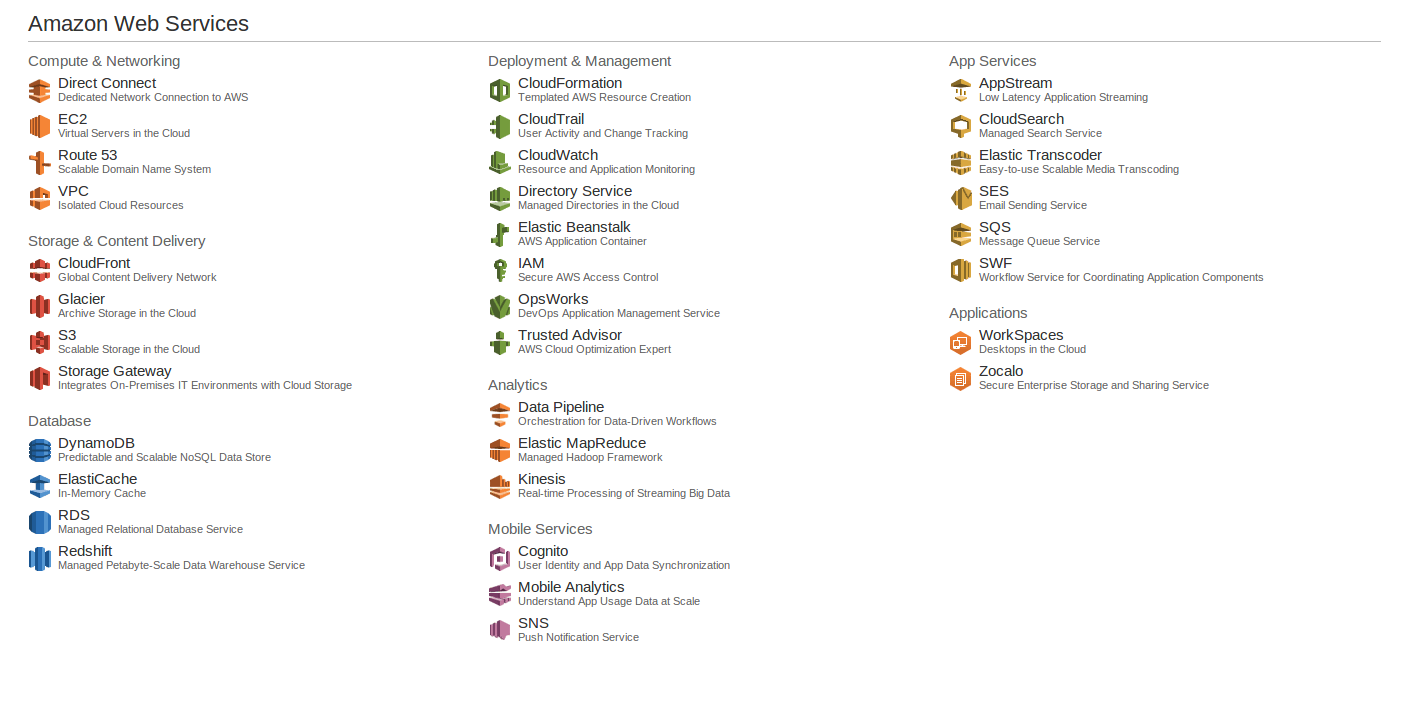
\includegraphics[width=1\textwidth]{img/aws_servicos}
    \end{center}
    \caption{Serviços da Amazon Web Services}
    \label{fig:aws_servicos}
\end{figure}

\begin{figure}[htp]
    \begin{center}
    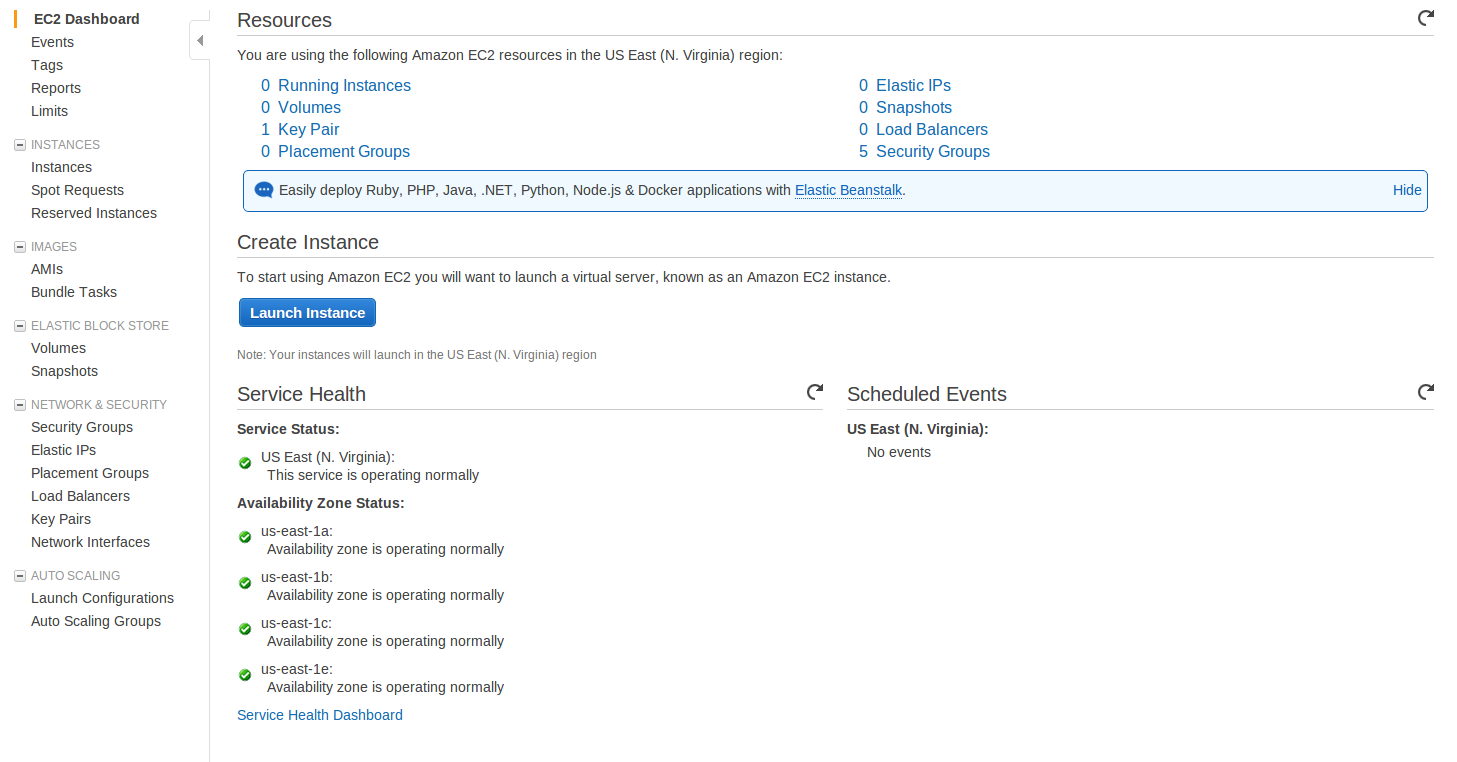
\includegraphics[width=1\textwidth]{img/aws_ec2}
    \end{center}
    \caption{Serviços de Elastic Compute Cloud (EC2)}
    \label{fig:aws_ec2}
\end{figure}

\begin{figure}[htp]
    \begin{center}
    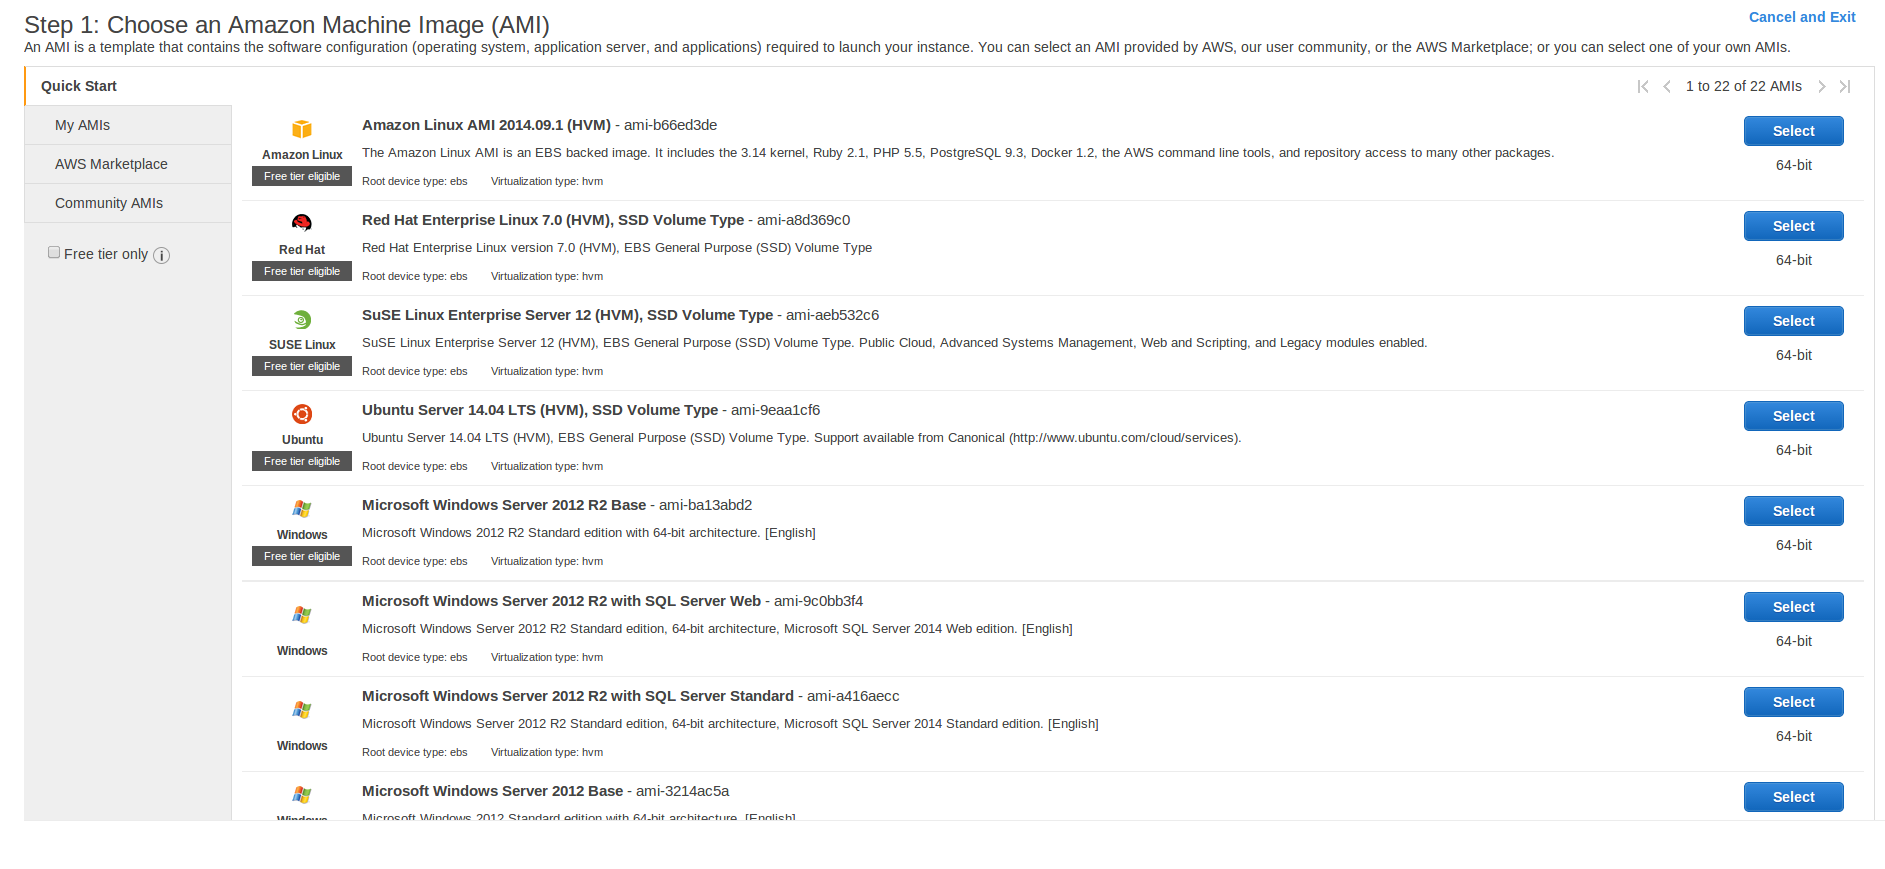
\includegraphics[width=1\textwidth]{img/aws_setup_ec2}
    \end{center}
    \caption{Escolha do tipo de configuração do software da máquina}
    \label{fig:aws_setup_ec2}
\end{figure}

\begin{figure}[htp]
    \begin{center}
    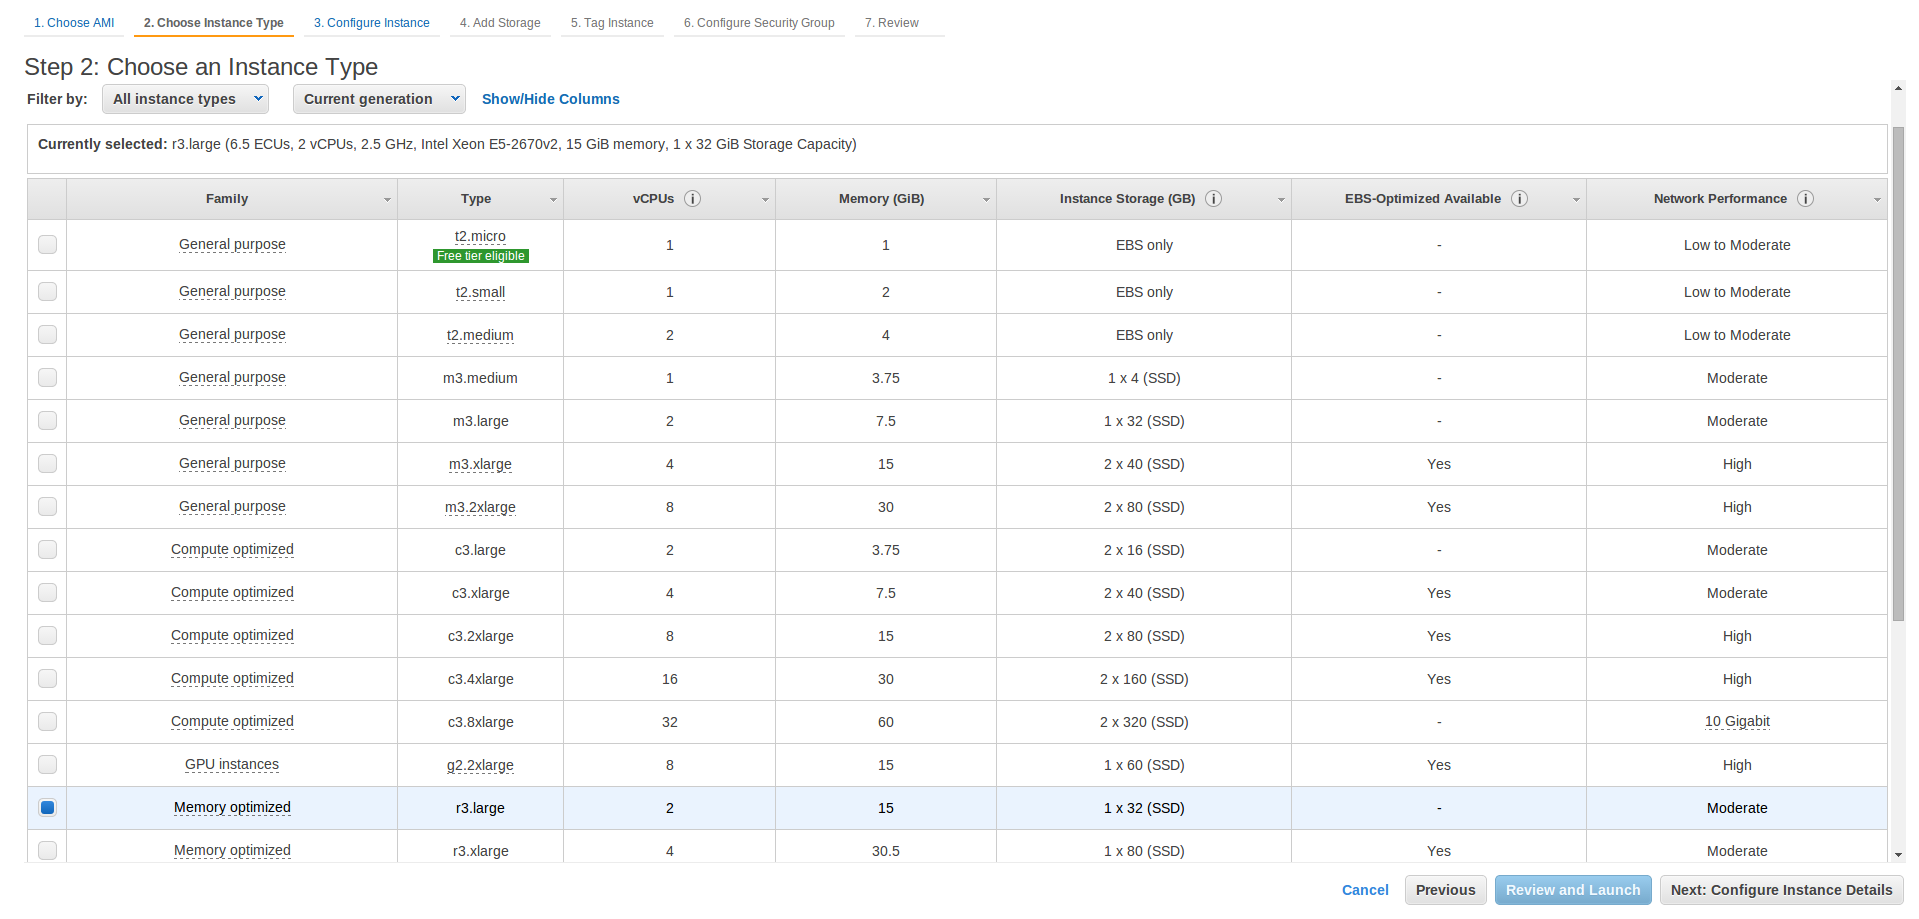
\includegraphics[width=1\textwidth]{img/aws_setup_ec2_maquina}
    \end{center}
    \caption{Escolha do tipo máquina}
    \label{fig:aws_setup_ec2_maquina}
\end{figure}

\begin{figure}[htp]
    \begin{center}
    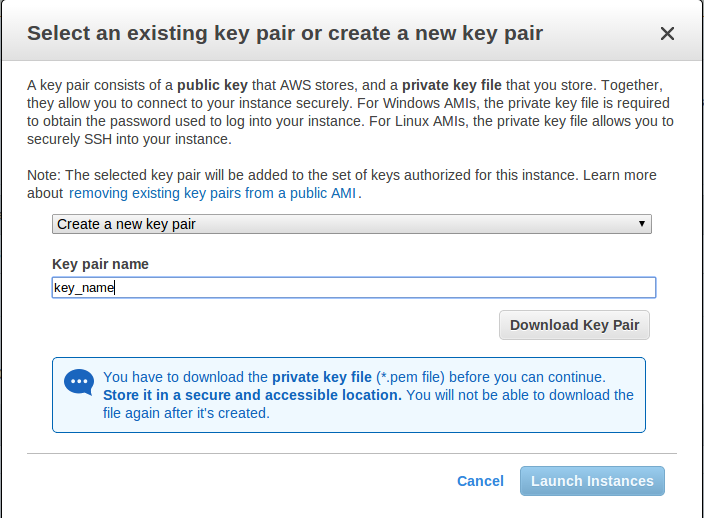
\includegraphics[width=1\textwidth]{img/aws_setup_keypair}
    \end{center}
    \caption{Criação da chave privada}
    \label{fig:aws_setup_keypair}
\end{figure}

\begin{figure}[htp]
    \begin{center}
    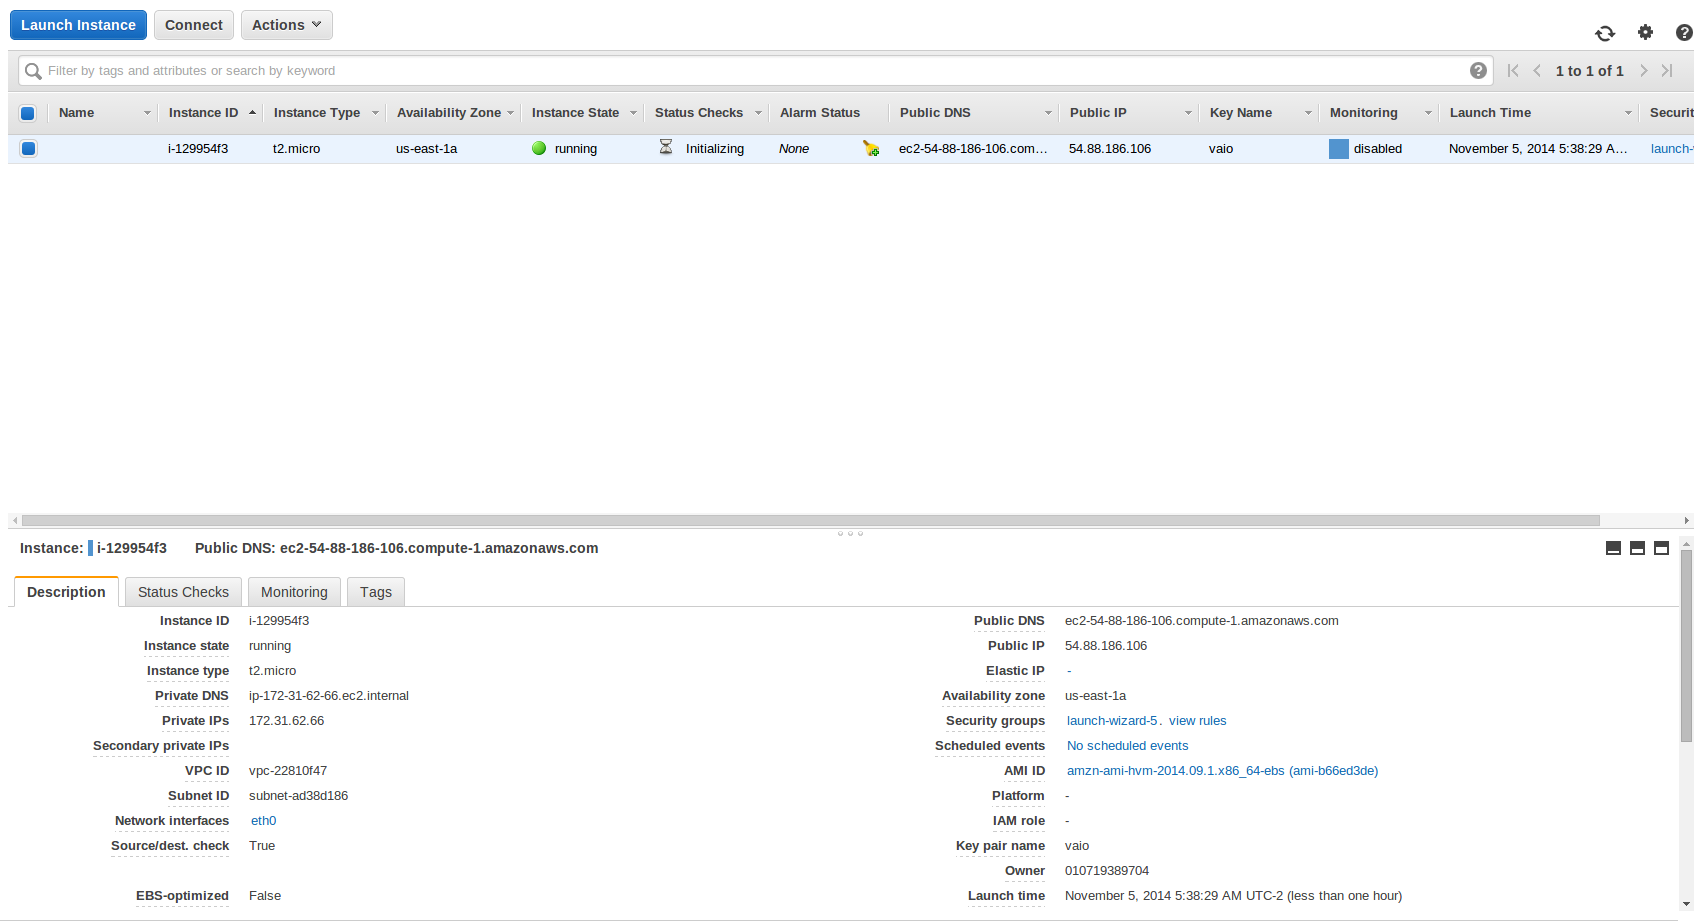
\includegraphics[width=1\textwidth]{img/aws_setup_dns}
    \end{center}
    \caption{Criação da máquina e do DNS público \textit{(Public DNS)}}
    \label{fig:aws_setup_dns}
\end{figure}



Uma vez criada a máquina, deve-se utilizar a chave privada para realizar um \textit{secure shell} e conectar-se remotamente ao EC2. A partir de um computador pessoal dotado de um interpretador de comandos \texttt{bash}, utilizamos a seguinte instrução:

\begin{lstlisting}[caption=Secure shell para conexão com a máquina virtual EC2]
ssh -i ~/Downloads/key_name.pem ec2-user@ec2-54-88-186-106.compute-1.amazonaws.com
\end{lstlisting}

Em seguida, para a automatização do ambiente de testes e rápida configuração de novas máquinas, criamos um arquivo \texttt{script.sh} na linguagem de programação \texttt{bash}. Esse \textit{script} instala os pacotes \texttt{R} e \texttt{git} e cria a chave pública necessária para acessar o servidor onde o código da biblioteca está hospedado. Em virtude de sua popularidade, utilizamos o serviço de hospedagem de códigos abertos GitHub (\url{https://github.com/aviggiano/tcc}). 

\begin{lstlisting}[caption=\textit{Script} de configuração do ambiente de testes]
#!/usr/bin/env bash
sudo su						# login como administrador. necessario para instalar pacotes no sistema operacional
yes | yum install R		# instala o pacote R no linux
yes | yum install git	# instala o git para descarregar os metodos de recomendacao
ssh-keygen -t rsa			# gera a chave para conectar-se ao GitHub
cat ~/.ssh/id_rsa.pub	# imprime a chave publica, que deve ser adicionada nas configuracoes do GitHub
\end{lstlisting}

A saída do \textit{script} é uma chave no seguinte formato:

\begin{lstlisting}[caption=Chave pública]
ssh-rsa AAAAB3NzaC1yc2EAAAADAQABAAABAQC/bxcszoyHzwyqtTXp4fl1Q3OT58Lsb7QLx+7nQ6
y0OIoWhK+r5ynSVi0BpTC+2hMrlg1rZTC1ED7Nb+SI9bRvf+1UYWOiVUXtwAVColMNBdIfE7QCWbJm
TmmBLcv9PIoCAvCfrxBh+flW3hXG388/LIEjZJckPYogho0jPAnFv3IXAGtVniV6cBcTTfKPUnX+np
6xiqnf4tYQpmPW/mnxk9s3bbEmcE1eYJkrE2IWdzy6EBnR9D4cBW5D8/VMM54xMJzugWZO//sIjLLT
0oFTTrroiwr+OX2DxqFdgCy8Agx1WZTeGhBAW1nvIVr5WVcWVBSzBCZfg8mYe+zYnbwl ec2-user@
ip-10-168-40-38
\end{lstlisting}

Após a obtenção da chave, deve-se cadastrá-la na página correspondente do GitHub (\url{https://github.com/settings/ssh}), como mostra a Figura \ref{fig:github_key}.

\begin{figure}[htp]
    \begin{center}
    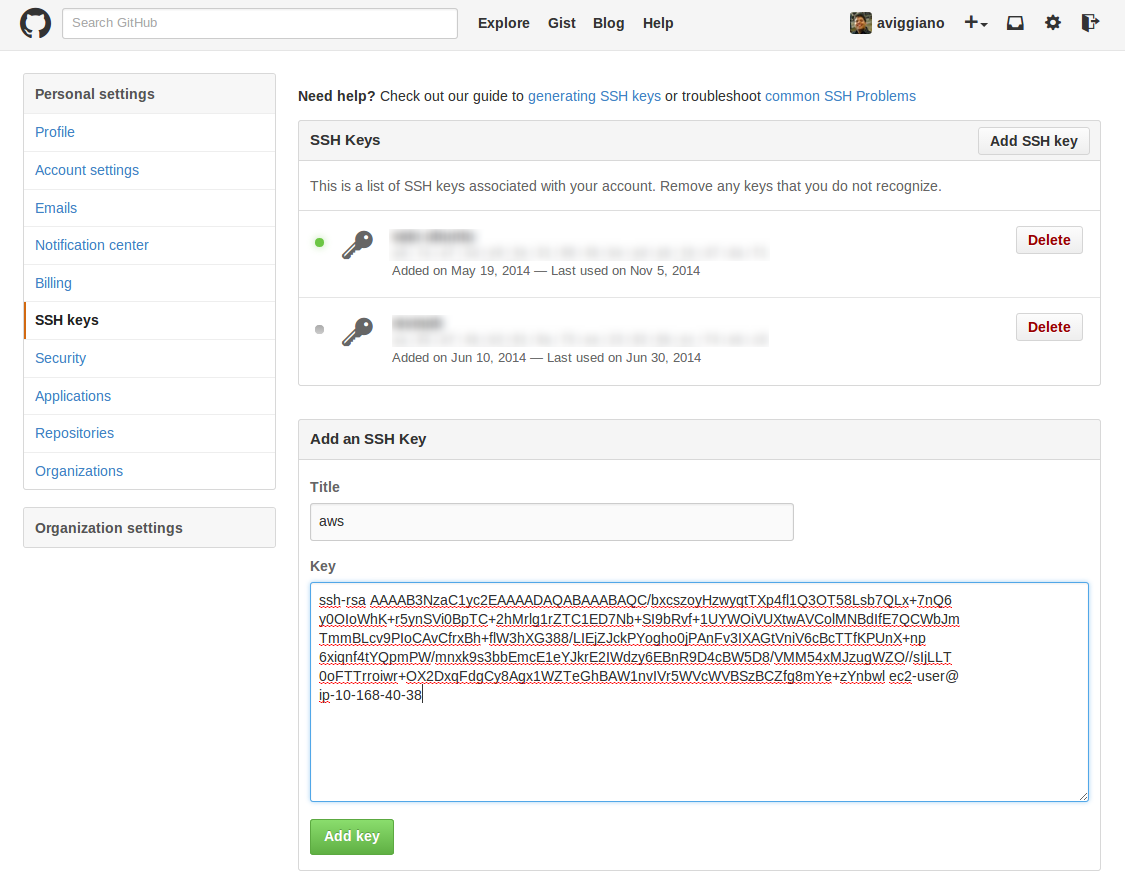
\includegraphics[width=1\textwidth]{img/github_key}
    \end{center}
    \caption{Cadastro da chave pública no GitHub}
    \label{fig:github_key}
\end{figure}

Uma vez tendo habilitado a máquina virtual da AWS para manipulação do repositório da biblioteca, pode-se descarregar o código e executar o \textit{script} de testes de qualidade:

\begin{lstlisting}[caption=Script de execução dos testes de qualidade]
#!/usr/bin/env bash
git clone git@github.com:aviggiano/tcc	# clona o repositorio
cd tcc && Rscript recsys/results/run_tests.R 		# executa o script de testes
\end{lstlisting}